\chapter{System Architecure} % Main chapter title

\label{Chapter3} % For referencing the chapter elsewhere, use \ref{Chapter1} 

The Complete System Architecture has been divided into following modules: Sensing Module, Controlling and Processing Module, Communication Module and Power Module.

\section{Sensing Module}
A sensor is a electronic device that generates signals upon detecting/sensing any physical conditions or chemical compounds, it's designed to detect. It is also defined as any device that converts a signal from one form to another. These are built with mostly electrical or electronic components. Our Sensing Unit comprises of sensors measuring different air-pollutants present in the air such as Nitrogen Oxide, Sulphur Dioxide, Carbon Monoxide, Carbon dioxide, and Particulate Matter.

\subsection{Sensor Description}
We have made our environment monitoring box with both High Quality Gas sensors as well as Low quality Gas sensors. They are used to make the device more robust, portable, sensitive, reliable and at the time cheaper.

\subsubsection{Low Quality Sensor}
We started our work with Environment Monitoring Box with some low quality sensors which are readily available and are incapable of measuring pollutants accurately but approximately. They give an indication of increase in pollutant level. They have a longer heating time and are less sensitivity. We have used the following semiconductor type Gas sensors:
\\
\\
\begin{enumerate}
	\item Semiconductor type Gas sensor: These devices are made up of heated metal oxides which are used for measurement of gas concentration of a target gas by measuring the electrical resistance of the device.
	\begin{itemize}
		\item \textbf{MQ-135}: It is used in air quality monitoring equipments for buildings/offices , suitable for detecting of $NH_3$, $NO_x$, alcohol, benzene, smoke, $CO_2$, etc. This sensor is composed of micro $Al_2O_3$ ceramic tube, Tin Dioxide ($SnO_2$) sensing layer, measuring electrode and a heater which are fixed into a crust made by plastic and stainless steel nets. The heater generates necessary conditions for working of the sensing component. The enveloped MQ-135 has 6 pins, 4 of them are used to fetch signals, and other two are used for providing heating current. Resistance value of MQ-135 is different for various kinds and various concentration of gases. While using these components, sensitivity adjustment was made. We calibrated the detector for 100ppm of $NH_3$ or 50ppm alcohol concentration in air and used value of Load Resistance(RL) about 20K (10K to 37K). The proper critical point for the gas detector was determined after considering the temperature and humidity influence.\\
		
		\begin{figure}[h]
		\centering
		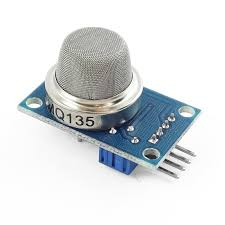
\includegraphics[width=0.3\textwidth]{./mq135}\\[0.1in]
		\label{sensor MQ135}
		\end{figure}
		
		\item \textbf{MQ-7}: It is used to detect Carbon Monoxide in the atmosphere. It is also composed of micro $Al_2O_3$ ceramic tube, Tin Dioxide ($SnO_2$) sensing layer, measuring electrode and heater which are fixed into a crust made by plastic and stainless steel nets. The enveloped MQ-7 has 6 pins, 4 of them are used to fetch signals, and other two are used for providing heating current. Standard measuring circuit of MQ-7, sensing component consist of 2 part, one is heating circuit having time control function (the high voltage and the low voltage work in loop) and the other is the signal output circuit that can accurately respond changes of surface resistance of the sensors.
				\\
				\begin{figure}[h]
				\centering
				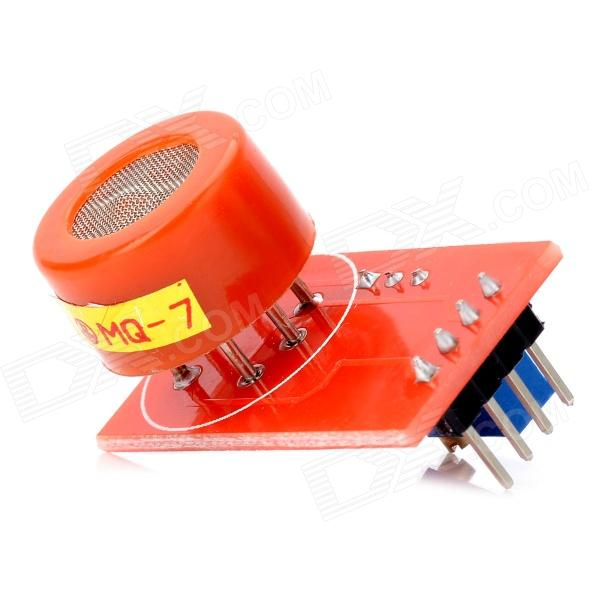
\includegraphics[width=0.3\textwidth]{./mq}\\[0.1in]
				\label{MQ7}
				\end{figure}
		\item \textbf{DHT11}: It features a temperature humidity sensor complexed with calibrated digital signal output. By using the exclusive digital-signal-acquisition technique and temperature humidity sensing technology, it ensures high reliability and excellent long term stability. This sensor includes a resistive type humidity measurement component and an NTC temperature measurement component, and connects to a high performance 8-bit micro-controller, offering excellent quality, fast response, anti-interference ability and also cost-effectiveness.
		\begin{figure}[h]
		\centering
		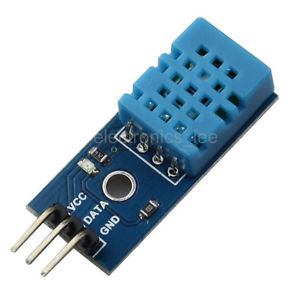
\includegraphics[width=0.3\textwidth]{./DHT11}\\[0.1in]
		\label{DHT11}
		\end{figure}
	\end{itemize}
	
	%\begin{figure}
	%\centering
	%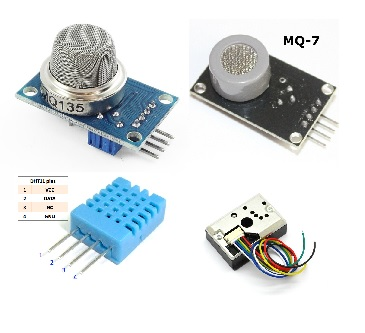
\includegraphics[width=0.8\textwidth]{./sensor}\\[0.1in]
	%\caption{Gas sensors}
	%\label{fig:Gas sensors}
	%\end{figure}

	

	\textbf{Working Principle (Semiconductor Gas Sensor)} : The detection principle of resistive sensors is based on change of the resistance of a thin film upon absorption of the gas molecules on the surface of semi-conductor. The gas-solid interactions affect the resistance of the film because of the density of electronic species in the film. Gas sensor is a subclass of chemical sensors.
\\
\\
Gas sensors measure the concentration of gases in its vicinity. It interacts with a gas to measure it's concentration. Each gas has a unique breakdown voltage i.e. the electric field at which it is ionized. Sensor identifies gas by measuring these voltages. The concentration of the gas can be determined by measuring the current discharge in the device.
\\
\\
	\textbf{Process Flow}:
	\begin{enumerate}
		\item Voltage supply to the sensor.
		\item Ceramic tube made up of $Al_2O_3$ heats up.
		\item Semiconductor chips conductivity is changed due to heating.
		\item Resistance of the circuit changes due to the presence of gas.
		\item Concentration of the gas is calculated by measuring the current since each gas has an unique breakpoint voltage. 
	\end{enumerate}

	\item Optical gas sensors (Dust Sensors) : This type of sensors uses optical absorption/emission scattering of a gas species at defined optical wavelengths. It consists of a light emitting element, a photo detecting element, a gas sensing element responding to light and a filter for picking up fluorescence or phosphorescence. Most optical sensors are usually based on thin films of palladium or chemo chromic oxides coated along the length of an optical fibre. This type of fibre optic sensors are known as optodes. Following methods are used by Optical Sensors\\
	 %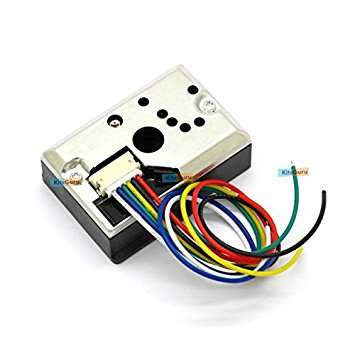
\includegraphics[width=0.8\textwidth]{./dust}\\[0.1in]
	
	\begin{itemize}
		\item Ellipsometry (Technique for the investigation of the dielectric properties)
		\item Spectroscopy (luminescence, phosphorescence, fluorescence, Raman)
		\item Interferometry (white light Interferometry, modal Interferometry in optical waveguide structures)
	\end{itemize}

	In these sensors a desired quantity is determined by:
	\begin{itemize}
		\item Refractive index (speed of light)
		\item Absorbance
		\item Fluorescence properties (of the analyse molecules or a chemo-optical transducing element)
	\end{itemize}

	\textbf{GP2Y1010AU0F} is a dust sensor built on optical sensing system. An infrared emitting diode (IRED) and a phototransistor are diagonally arranged into this device. It detects the reflected light of dust in air. It is effective to detect very fine particle like cigarette smoke.
\begin{figure}
\centering
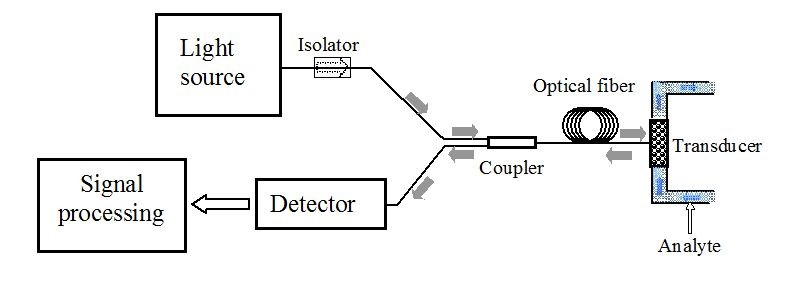
\includegraphics[width=0.8\textwidth]{./optical}\\[0.1in]
\label{fig: Optical sensor}
\caption{Optical sensor}
\end{figure}

	\textbf{Working Principle (Optical Sensors)}:
	\begin{enumerate}
		\item Dust enters through the hole of the sensors.
		\item Infrared emission take place through the IRED.
		\item Reflection of light through dust particles takes place.
		\item As Photo transistor is diagonally arranged to the IRED it gets activated by the refraction. 
		\item The resistance of the Amplifier circuit changes which in turn changes the output voltage.
		\item The concentration of dust is measured by the change in output voltage. 
	\end{enumerate}

\end{enumerate}

\subsubsection{Hight Quality Sensors}
These are the sensors which give stable and more accurate reading with less noise. Following are the Sensors that we have used during our project:

\begin{enumerate}
	\item \textbf{Multichannel Gas Sensor}: It is a built with MiCS-6814 which can detect many unhealthy gases, and three gases can be measured simultaneously due to its three channels, so it can help you to monitor the concentration of more than one gas.  This sensor belongs to Grove System, and you can plug it onto the Grove Base Shield and work with Arduino directly without any jumper wires. It as an I2C interface.

\begin{figure}[h]
	\centering
	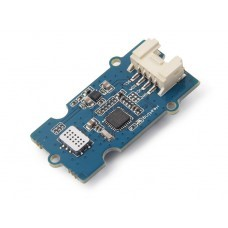
\includegraphics[width=0.4\textwidth]{./multi}\\[0.1in]
	\label{fig:Multichannel gas sensor}
	\caption{Multichannel gas sensor}
	\end{figure}


	\textbf{Detectable Gasses}:
		\begin{itemize}
			\item Carbon monoxide CO (1$-$1000)ppm
			\item Nitrogen dioxide $NO_2$ ( 0.05$-$10 )ppm
			\item Ethanol $C_2H_6$OH (10$–$500)ppm
			\item Hydrogen $H_2$ (1$-$1000)ppm
			\item Ammonia $NH_3$ (1$-$500)ppm
			\item Methane $CH_4$ ($>$1000)ppm
			\item Propane $C_3H_8$ ($>$1000)ppm
			\item Iso-butane $C_4H_{10}$ ($>$1000)ppm
		\end{itemize}
	(Mainly we have used this sensor to measure the concentration of CO and $NO_2$)
	\item Grove – Temperature \& Humidity Sensor (High-Accuracy \& Mini) v1.0: This is a multifunctional sensor that gives you temperature and relative humidity information at the same time. It utilizes a TH02 sensor that can meet measurement needs of general purposes. It provides reliable readings when environment humidity condition in between 0-80\% RH, and temperature condition in between 0-70°C, covering needs in most of the household and daily applications that doesn't reach extreme conditions.
	\\
	\begin{figure}[h]
	\centering
	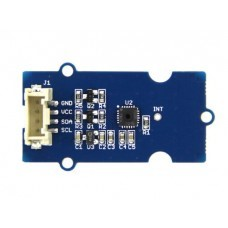
\includegraphics[width=0.4\textwidth]{./temp}\\[0.1in]
	\label{fig:temperature and Humidity sensor}
	\caption{temperature and Humidity sensor}
	\end{figure}
	
	\item PM Dust Sensor Module – Laser Sensing: It is a universal particle concentration measurement digital sensor used to obtain the number of suspended particulate matter in a unit volume of air within 0.3 to 10 microns (concentration of particulate matter) and output with digital interface, also can output quality data of per particle. These sensors can be used in a variety of environmental conditions where it provides timely and accurate concentration data.
\\
\\
	\textbf{Detectable Particulate Matters}: Can detect Particulate Matter of Size 1 Micron, 2.5 Micron and 10 Micron.
\end{enumerate}

\section{Controlling and Processing Unit}

\textbf{A microcontroller} is a small and low-cost microcomputer, which is designed to perform the specific tasks of embedded systems like displaying microwave’s information, receiving remote signals, etc.
\\
\\
\textbf{A microprocessor} is a computer processor which incorporates the functions of a computer's central processing unit (CPU) on a single integrated circuit (IC), [1] or at most a few integrated circuits. [2] The microprocessor is a multipurpose, clock driven, register based, digital-integrated circuit which accepts binary data as input, processes it according to instructions stored in its memory, and provides results as output. Microprocessors contain both combinational logic and sequential digital logic. Microprocessors operate on numbers and symbols represented in the binary numeral system.
\\
\\
\textbf{Difference between Microprocessor \& Microcontroller}:

\begin{center}
 \begin{tabular}{| c |  p{6cm} | p{6cm} |} 
 \hline
 Sl. & Microcontroller & Microprocessor \\ [0.5ex] 
 \hline\hline
 1 & It doesn’t consist of RAM, ROM, I/O ports. It uses its pins to interface to peripheral devices. & It consists of CPU, RAM, ROM, I/O ports. \\ 
 \hline
 2 & Microcontrollers are used to execute a single task within an application. &  Microprocessors are used for big applications. \\
 \hline
 3 & Its designing and hardware cost is low. & Its designing and hardware cost is high. \\
 \hline
 4 & Easy to replace. & Not so easy to replace. \\
 \hline
 5 & It is built with CMOS technology, which requires less power to operate. & Its power consumption is high because it has to control the entire system. \\
 \hline
\end{tabular}
\end{center}

\begin{enumerate}
	\item \textbf{Arduino Mega 2560}: The Mega 2560 is a microcontroller board based on the ATmega2560. It has 54 digital input/output pins (of which 15 can be used as PWM outputs), 16 analog inputs, 4 UARTs (hardware serial ports), a 16 MHz crystal oscillator, a USB connection, a power jack, an ICSP header, and a reset button. It contains everything needed to support the microcontroller; simply connect it to a computer with a USB cable or power it with a AC-to-DC adapter or battery to get started. 

\begin{center}
 \begin{tabular}{| c |  p{6cm} | p{6cm} |} 
 \hline
 Sl. & Microcontroller & Microprocessor \\ [0.5ex] 
 \hline\hline
 1 & Operating Voltage & 5V \\ 
 \hline
 2 & Input Voltage (recommended) & 7-12V \\
 \hline
 3 & Input Voltage (limit) & 6-20V \\
 \hline
 4 & Digital I/O Pins & 54 (of which 15 provide PWM output) \\
 \hline
 5 & Analog Input Pins & 16 \\
 \hline
6 & DC Current per I/O Pin & 20 mA \\
 \hline
7 & DC Current for 3.3V Pin & 50 mA \\
 \hline
8 & Flash Memory Pin & 256 KB of which 8 KB used by bootloader \\
 \hline
9 & SRAM & 8 KB \\
 \hline
10 & EEPROM & 4 KB \\
 \hline
11 & Clock Speed & 16 MHz \\
 \hline
12 & Length & 101.52 mm \\
 \hline
13 & Width & 53.3 mm \\
 \hline
14 & Weight & 37 g \\
 \hline
\end{tabular}
\end{center}

\textbf{Programming}: The Mega 2560 board can be programmed with the Arduino Software (IDE).The ATmega2560 on the Mega 2560 comes pre-programmed with a bootloader that allows you to upload new code to it without the use of an external hardware programmer. It communicates using the original STK500 protocol (reference, C header files).
\begin{figure}
\centering
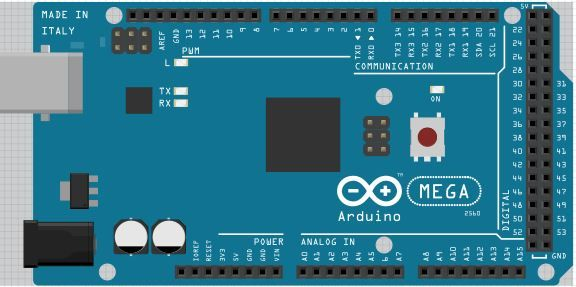
\includegraphics[width=0.6\textwidth]{./arduino}\\[0.1in]
\label{fig:Arduino Mega 2560}
\caption{Arduino Mega 2560}
\end{figure}


\textbf{Warnings}: The Mega 2560 has a resettable poly-fuse that protects your computer's USB ports from shorts and overcurrent. Although most computers provide their own internal protection, the fuse provides an extra layer of protection. If more than 500 mA is applied to the USB port, the fuse will automatically break the connection until the short or overload is removed.
\\
\\
\textbf{Power}: The Mega 2560 can be powered via the USB connection or with an external power supply. The power source is selected automatically. External (non-USB) power can come either from an AC-to-DC adapter (wall-wart) or battery. The adapter can be connected by plugging a 2.1mm centre-positive plug into the board's power jack. Leads from a battery can be inserted in the GND and Vin pin headers of the POWER connector.
\\
\\
The board can operate on an external supply of 6 to 20 volts. If supplied with less than 7V, however, the 5V pin may supply less than five volts and the board may become unstable. If using more than 12V, the voltage regulator may overheat and damage the board. The recommended range is 7 to 12 volts.
\\
\\
\textbf{Memory}: The ATmega2560 has 256 KB of flash memory for storing code (of which 8 KB is used for the bootloader), 8 KB of SRAM and 4 KB of EEPROM.
\\
\\
\textbf{Communication}: The Mega 2560 board has a number of facilities for communicating with a computer, another board, or other microcontrollers. The ATmega2560 provides four hardware UARTs for TTL (5V) serial communication. An ATmega16U2 (ATmega 8U2 on the revision 1 and revision 2 boards) on the board channels one of these over USB and provides a virtual com port to software on the computer (Windows machines will need a .inf file, but OSX and Linux machines will recognize the board as a COM port automatically.
\\
\\
 The Arduino Software (IDE) includes a serial monitor which allows simple textual data to be sent to and from the board. The RX and TX LEDs on the board will flash when data is being transmitted via the ATmega8U2/ATmega16U2 chip and USB connection to the computer (but not for serial communication on pins 0 and 1).

\item \textbf{Raspberry Pi 3 Model B}: 
A Raspberry Pi is a credit card-sized computer originally designed for education, inspired by the 1981 BBC Micro. Creator Eben Upton's goal was to create a low-cost device that would improve programming skills and hardware understanding at the pre-university level. But thanks to its small size and accessible price, it was quickly adopted by tinkerers, makers, and electronics enthusiasts for projects that require more than a basic microcontroller (such as Arduino devices).
\\
\\
The Raspberry Pi is slower than a modern laptop or desktop but is still a complete Linux computer and can provide all the expected abilities that implies, at a low-power consumption level.
\\
\\
The Raspberry Pi is open hardware, with the exception of the primary chip on the Raspberry Pi, the Broadcom SoC (System on a Chip), which runs many of the main components of the board–CPU, graphics, memory, the USB controller, etc. Many of the projects made with a Raspberry Pi are open and well-documented as well and are things you can build and modify yourself.
\\
\\
The Raspberry Pi was designed for the Linux operating system, and many Linux distributions now have a version optimized for the Raspberry Pi. Two of the most popular options are Raspbian, which is based on the Debian operating system, and Pidora, which is based on the Fedora operating system.
\begin{figure}
\centering
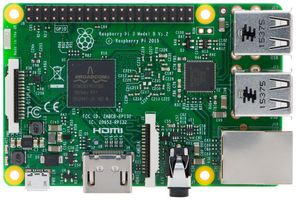
\includegraphics[width=0.6\textwidth]{./pi}\\[0.1in]
\label{fig:Raspberry pi}
\caption{Raspberry pi}
\end{figure}


\textbf{Specification}:
\begin{itemize}
	\item \textbf{SoC}: Broadcom BCM2837 (roughly 50\% faster than the Pi 2)
	\item \textbf{CPU}: 1.2 GHZ quad-core ARM Cortex A53 (ARMv8 Instruction Set)
	\item \textbf{GPU}: Broadcom VideoCore IV @ 400 MHz
	\item \textbf{Memory}: 1 GB LPDDR2-900 SDRAM
	\item \textbf{USB ports}: 4
	\item \textbf{Network}: 10/100 MBPS Ethernet, 802.11n Wireless LAN, Bluetooth 4.0
\end{itemize}

\item \textbf{Additional Component}:
We have used our sensors to gather data and microcontroller (Arduino mega 2560) to control the flow of data but we need to get the real time data of a place and also we need to store the data for data analysis.
\\
\\
\textbf{RTC (Real Time Clock)}: A real-time clock (RTC) is a computer clock (most often in the form of an integrated circuit) that keeps track of the current time. To get the time of a data we have connected RTC with the Arduino mega 2560.
\begin{figure}
\centering
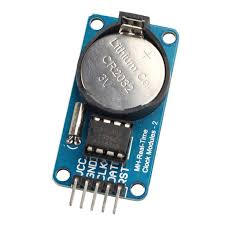
\includegraphics[width=0.3\textwidth]{./rtc}\\[0.1in]
\label{fig: RTC}
\caption{RTC}
\end{figure}

\textbf{SD Card Module and Micro SD card}: SD card module takes the sensor data from the Arduino mega 2560 and store it into the SD card for permanent data storage for further analysis of data. 
\end{enumerate}
%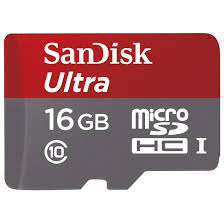
\includegraphics[width=0.5\textwidth]{./microsd}\\[0.1in]
%\label{Microsd card }




\section{Communication Module}
%VIVEK's PART
\subsection{Architecture}
The data from the Sensors is received by the Arduino Mega 2560 is transferred to the Raspberry Pi(Microprocessor) via serial Communication (Tx and Rx). Data is stored in the memory of Raspberry Pi for further communication. Raspberry Pi is having Bluetooth and WiFi for communication. The Raspberry Pi is Connected to the Internet via Wifi. Data from the raspberry pi send to the firebase database using Firebase API.
Android application is used to fetch the data stored on cloud . Firebase is real time database , Android application fetch the real time data from cloud using Firebase API.Output display the output on the student screen.  

\begin{figure}[!htbp]
	\centering
	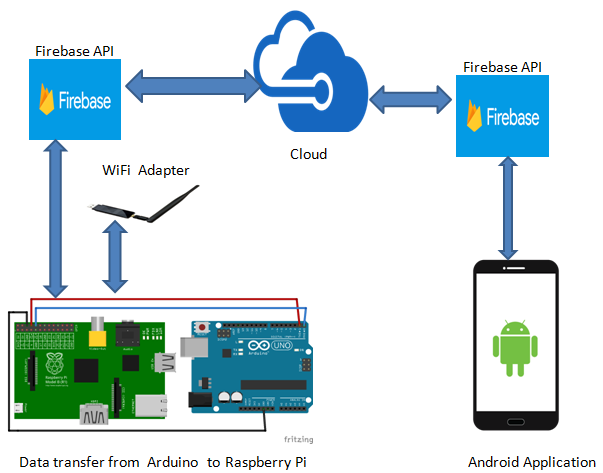
\includegraphics[width=0.9\textwidth]{image1.png}
	\label{fig:Architecture}
	\caption{Architecture}
\end{figure}
 

\subsection{Working of Android Application}

Application needs permission from different hardware, software, internet or any other resource it uses to complete the task. In this application there are four parameter namely Current-Pollution-Status where user can see the current concentration of the pollution of the classroom, Create-Profile where student can create their own profile, view-profile where student can select their profile and compare profile data with the current data of pollutant concentration present in the classroom and Student-Survey in this form student can give their feedback and status of the classroom.
\begin{figure}[!htbp]
	\centering
	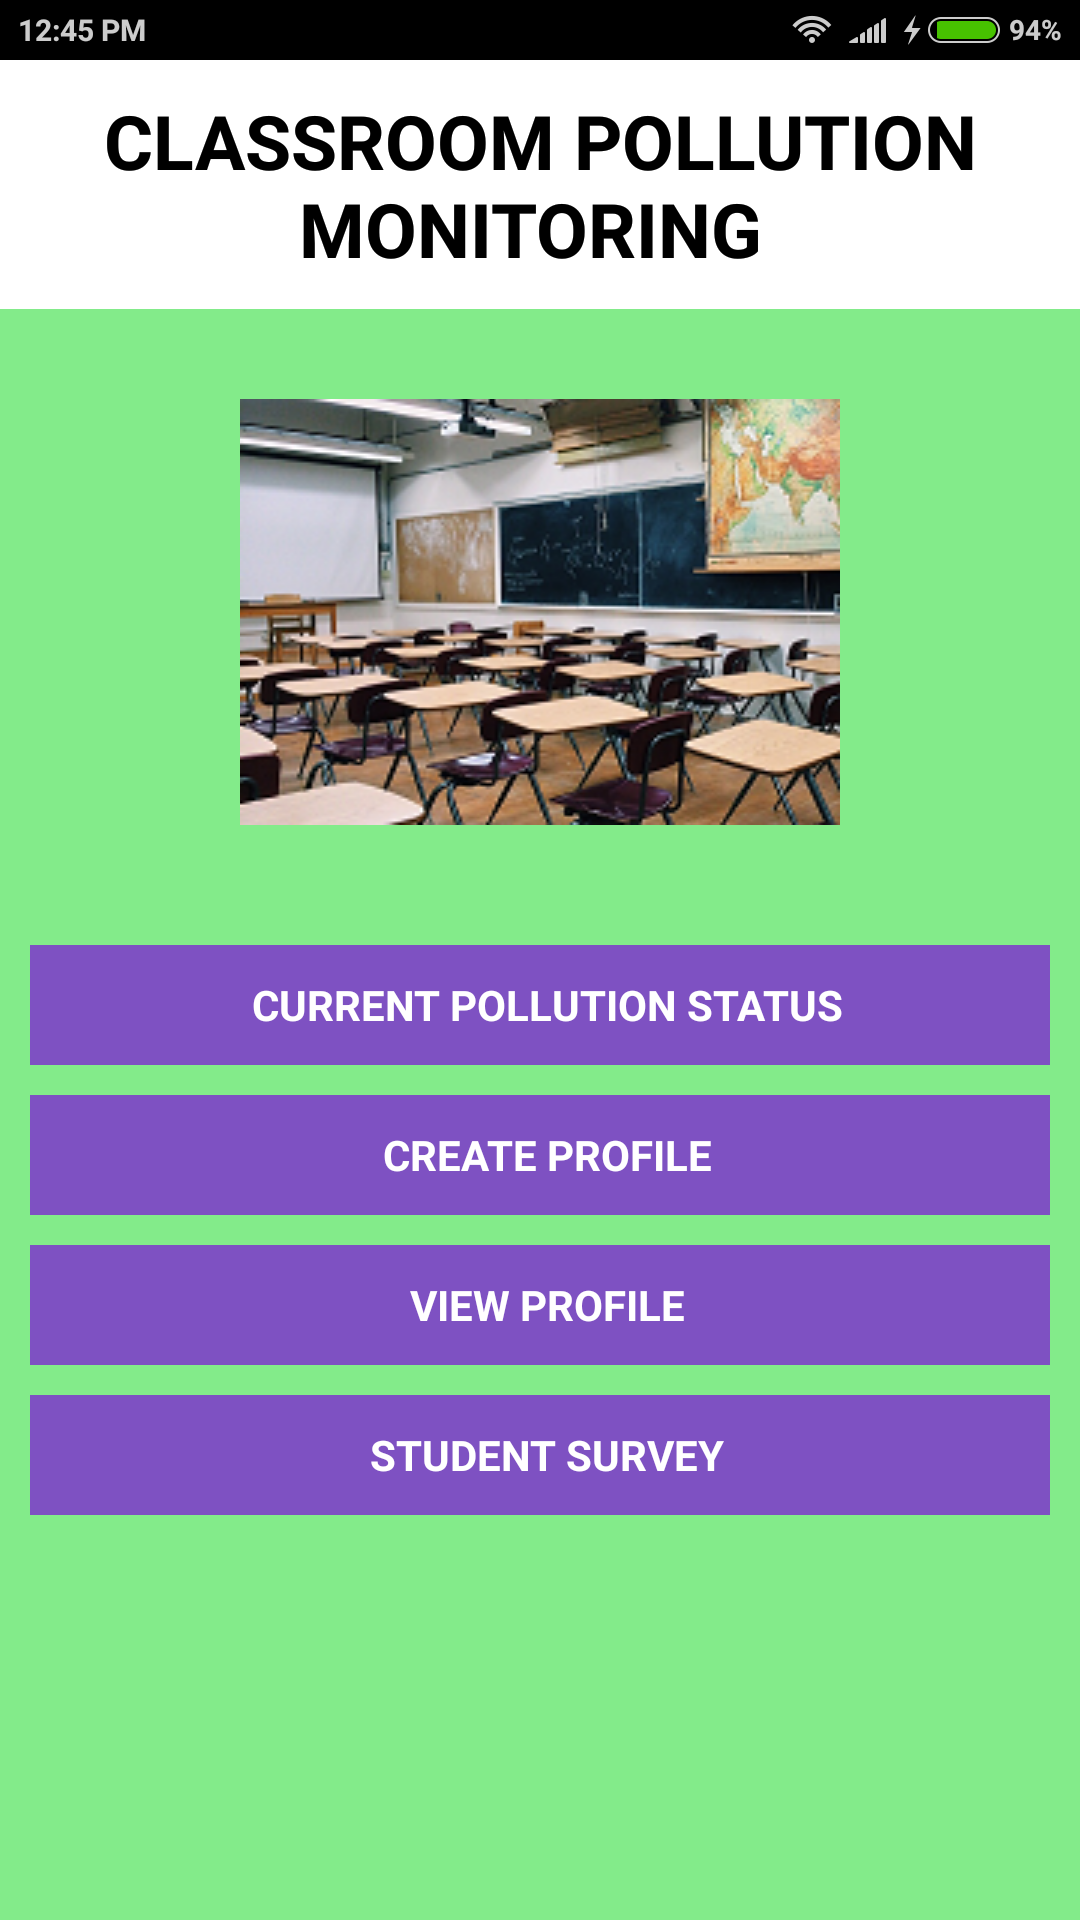
\includegraphics[scale=0.09]{image2.png}
	\label{fig:Working of Android App}
	\caption{Working of Android App}
\end{figure}

\section{Power Module}
The prototype Box can run on AC main power supply current and is also backed up with a 12 V 12 A Battery for load shedding. The Sensors and Microcontrollers require 5 V DC power supply. So we have designed a circuit that will convert the 220 V AC to 5 V DC for smooth running of the device without any power problem.
\\
\\
Also we have installed a 12 V 12 A dry cell battery for power back up.
\\
\\
Sensors and device power used specification.
\\
\\
\begin{center}
 \begin{tabular}{| c |  p{4cm} | p{3cm} | p{3cm} | p{3cm} |} 
\hline
 Sl. & Sensor & Voltage & Current & Power = V * I \\ [0.5ex] 
 \hline\hline
 1 & Arduino Mega 2560 & 5V & 200mA & 1 W \\ 
 \hline
 2 & Laser dust sensor: SKU:SEN0177 & 5V & 200mA & 1 W \\
 \hline
 3 & Temperature and Humidity (TH02) & 5V & 350 micro-A & 1.75 mW \\
 \hline
 4 & Grove - Multichannel gas sensor & 5 V & 30 mA & 150 mW \\
 \hline
 5 & MQ-135 & 5 V & 160 mA & 800 mW \\
 \hline
6 & SD card Module & 5 V & 100 mA & 500mW \\
 \hline
7 & RTC & 5 V & 100 mA & 500 mW \\
 \hline
  &   &   &  \textbf{Total} & 3.95 W(approx 4 W) \\
 \hline
\end{tabular}
\end{center}

\textbf{Formula used}: $$Power = Voltage x Current$$
\\
\\
So we have calculated that our device is drawing approximately 4 W of current.
\\
\\
\textbf{Calculation of Time taken for batter to discharge}:
\\
\\
As we have mentioned that our device is batter enabled for load shedding so we have done a small calculation to find out the duration for the use of batter in case of emergency.
\\
\\
Battery:
\\
\\ 
The specifications of the battery are as follows: 

	$$Voltage = 12 V$$
	$$Current = 12 A$$
	
With the equation to find the power
	$$Power = Voltage x Current$$ \\
		
		$$Total Power of the battery is = (12 x 12) W$$
		$$= 144 W$$
\\
\\
Device:
\\
\\
	
From the above table the total power used by the box  = 4 W
\\
\\
Now we will calculate the time taken for the battery to discharge
$$Time = Battery power / Device power$$\\
	$$= 144 W / 4 W$$
	$$= 36 Hours $$
\\
\\
So our device will run for approximately 36 hours on battery too.

\vspace{0.4in}
\section {Prototype Device}
\vspace{0.2in}
With all these Components combined we have build our prototype device. We named our Device "Environment Monitoring System". The images of our prototype image are given below.
\begin{figure}[!htpb]

\begin{subfigure}
\centering
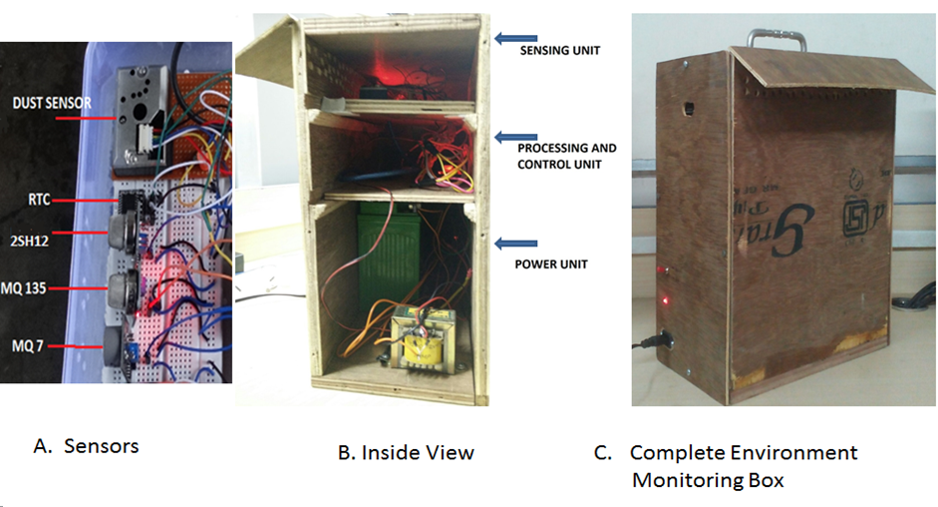
\includegraphics[width=0.8\textwidth]{./prototype_final}\\[0.1in]
\label{fig: Air Quality Monitoring Box}
\caption{AQM Box}
\end{subfigure}

\begin{subfigure}
\centering
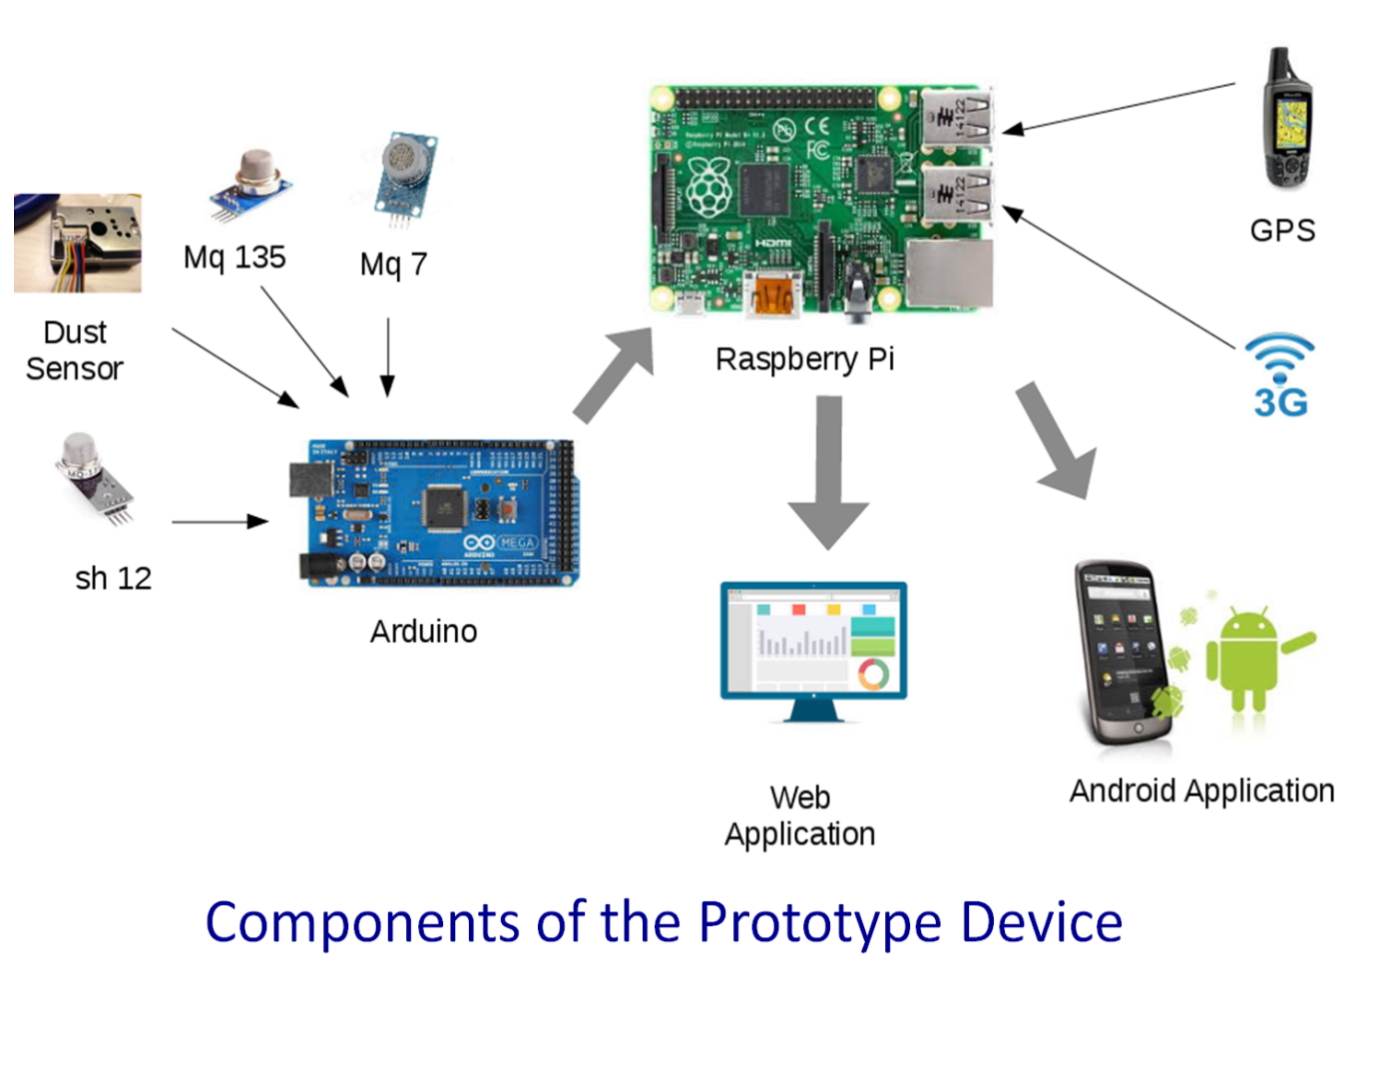
\includegraphics[width=0.8\textwidth]{./prototype_arch}\\[0.1in]
\label{fig: Air Quality Monitoring Box Architecture}
\caption{AQM Box Arch}
\end{subfigure}

\end{figure}